\documentclass[letterpaper,12pt,aps, pra]{revtex4-1}
\renewcommand{\baselinestretch}{1.0}
%\usepackage{times}
\usepackage{amsmath} \usepackage{subfigure} \usepackage{graphicx}
\usepackage{rotating}
\usepackage{multirow}
\usepackage{hyperref}
\usepackage{graphicx}
\usepackage{color}
\usepackage{verbatim}
\bibliographystyle{abbrv}

\usepackage{amsmath}
\begin{document}

\vfill
{\LARGE
  \begin{center}
{BLOCK}
\end{center}
}
\vspace{0.5in}
\begin{center}{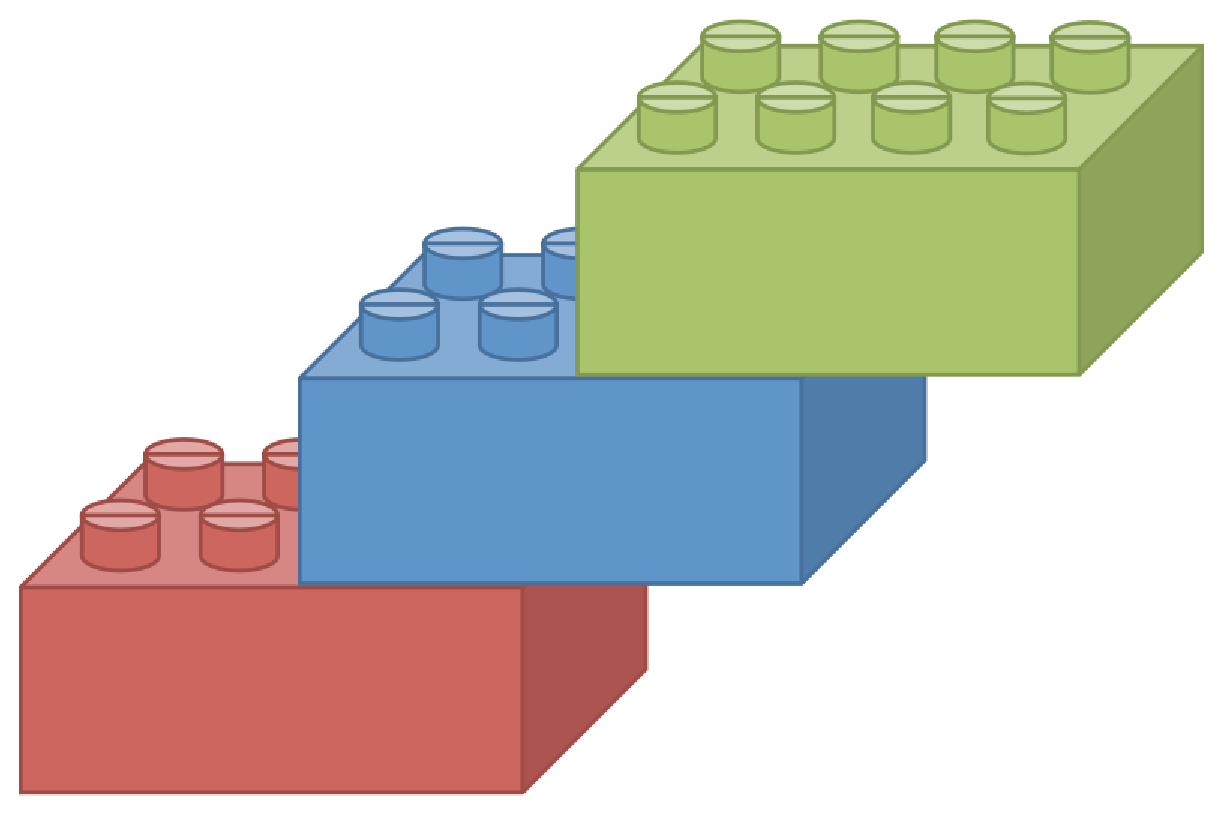
\includegraphics[width=2in]{block_logo}}\\
\end{center}
\vspace{0.5in}
\begin{center}
{\Large \textsc{version 1.0.0}}
\end{center}
\vspace{1in}

{\large
\begin{center}
Sandeep Sharma, Roberto Olivares-Amaya and Garnet Kin-Lic Chan\\
\vspace{0.2in}
with contributions from\\
\vspace{0.2in}
Jonathan Dorando and Debashree Ghosh
\end{center}
}
\vspace{1in}

\thispagestyle{empty}
\newpage

\pagenumbering{roman}
\tableofcontents
\newpage
\pagenumbering{arabic}

%\begin{comment}
%\section{Introduction}
\texttt{BLOCK} implements the density matrix renormalization group (DMRG) algorithm for quantum chemistry. 
The DMRG is a variational wavefunction method. Compared to other quantum chemical methods, 
{\it it  efficiently describes strong, multi-reference correlation in
 a large number of active orbitals (occupancies far from 0 or 2)}.
The method is also provably optimal for correlation with a one-dimensional topology, that is,
where orbitals are arranged with a chain- or ring-like connectivity.
However, with the possible exception of small molecules, for correlation that is dynamic in character, the DMRG may be less computationally
efficient than other methods such as coupled cluster theory or multireference configuration interaction.

We recommend the use of the DMRG in problems requiring active spaces too large for standard 
complete active space (CAS) techniques. Thus, if you are interested in
\begin{itemize}
\item a CAS-like treatment of low-lying eigenstates in problems with 16-40 active orbitals,
\item or, one-dimensional orbital topologies with up to 100 active orbitals,
\item and, standard chemical accuracy (1 kcal/mol in energy differences),
\end{itemize}
then the DMRG may be the right method for you.
%\end{comment}

\section{Capabilities}

As of the current 1.0.0 release, \texttt{BLOCK} implements the following features:
\begin{itemize}
\item DMRG sweep algorithm for quantum chemistry Hamiltonians,
\item Efficient warm-up algorithm for large systems (\ref{sec:warmup}),
\item Full spin-adaptation (SU(2) symmetry) and Abelian point-group symmetries,
\item State-averaged excited states (\ref{sec:AppSA}),
\item State-specific calculation (\ref{sec:AppSS}),
\item $n$-particle density matrices ($n\le4$) and transition density matrices ($n\le2$) (\ref{sec:AppNpdm}),
\item A convenient interface to the Molpro, ORCA and Q-Chem program packages.
\end{itemize}

\section{Installation}\label{sec:install}

\texttt{BLOCK} can either be built as a standalone or through one of its interfaces to external programs. Please Sec.~\ref{sec:External} for including \texttt{BLOCK} as an external library.

\subsection{MOLPRO}
\texttt{MOLPRO} fetches a copy of the most recent stable \texttt{BLOCK}
code, and compiles it. For this, the

\begin{verbatim}
-enable-Block
\end{verbatim}

flag must be called when running \begin{verbatim}./configure\end{verbatim}. Please refer to the Molpro manaul for more details.

\subsection{ORCA}

\texttt{BLOCK} is enabled in \texttt{ORCA} by enabling the flag \texttt{USE\_DMRG = YES} in the Makefile.

\subsection{Q-Chem}

\texttt{BLOCK} has been merged into \texttt{Q-Chem} package and is built automatically by compiling \texttt{Q-Chem 4.2.2} or later version.

\subsection{Standalone}
\texttt{BLOCK} is written in C++ and requires a C++ compiler. It has the following additional dependencies:
\begin{itemize}
\item Complete BLAS, LAPACK, and Boost C++ libraries,
\item For parallel execution MPI must be installed, and the Boost MPI library must have been compiled with the same version of MPI,
\item Depending on the operating system, you may wish to install a custom malloc (see Sec.~\ref{sec:appInstall}, and Sec. \ref{sec:computation}),
\item Python, to run the tests.
\end{itemize}
The program has been tested on Linux systems, although we expect it to run on other Unix type operating systems as well. 

%maybe switch to appendix
\subsubsection{makefile}
\texttt{BLOCK} is compiled using the makefile supplied in the distribution. The following customizations need to be made to the makefile. More details follow in Sec.~\ref{sec:appInstall}
\begin{itemize}
 \item \textbf{Boost}\\The variable \texttt{BOOST} should be set to the location of the Boost installation. 
\item \textbf{Lapack and Blas}\\ The variable \texttt{LAPACKBLAS} should be
set to the linking command for the BLAS and LAPACK libraries.
\item \textbf{Compiler}\\
   By default, \texttt{BLOCK} is set up to use the gcc compiler. If you wish to use the Intel C++ compiler you should modify the variable \texttt{CXX} to \texttt{icpc}.
\item \textbf{Parallel execution}\\
	is enabled by default. Make sure that the \texttt{MPI\_LIB} variable points to the location of the boost\_mpi library. If one wishes to use only the serial version of \texttt{BLOCK}, modify the \texttt{USE\_MPI} variable to \texttt{false}.
	If an mpi enabled c++ wrapper compiler ``mpic++'' is available then no further changes are necessary. If this is not the case then \texttt{MPICXX} should be changed to the name of the parallel C++ compiler.  Also in absence of the wrapper compiler additional mpi libraries need to be specified manually using the variable \texttt{MPI\_LIB}. %\texttt{CXX} should be changed to the name of the parallel C++ compiler or wrapper (e.g. mpic++). In general, the parallel wrapper will automatically link the appropriate MPI libraries. However, if MPI libraries need to be linked manually, \texttt{MPI\_LIB} should be set to the appropriate linking command.
%% To install the parallel version of the code the variable \textsf{USE\_MPI} should be set to \textsf{yes}. If an mpi enabled c++ wrapper compiler ``mpic++'' is available then no further changes are necessary. If this is not the case then one needs to manually change two entries, line 36 and line 37, of the makefile. Line 36 defines the variable \textsf{MPI\_LIB}. In addition to the linking Qcdmrg with the mpi boost library, additional mpi libraries need to be specified. The location of these will depend on the platform and also the flavor of mpi installed. Line 37 defines the variable \textsf{CXX} as \textsf{mpic++}; this has to be changed to the usual c++ compiler one is interested in using e.g. g++ for the case of gcc compiler.
\item \textbf{Custom malloc} \label{sec:appInstall}\\
DMRG calculations allocate and deallocate small blocks of memory a large number of times during a single calculation. For large scale calculations,
this can lead to significant memory fragmentation over time. In some cases, this can be significantly ameliorated by installing a
custom memory allocator. The linking command for the memory allocator is given by the variable \texttt{MALLOC},
\end{itemize}


\section{Running and testing the code}

The standalone code can be executed using the command
\begin{verbatim}
block.spin_adapted input.dat > output.dat
\end{verbatim}
\texttt{input.dat} is the input file and the output of the program is piped 
into the output file \texttt{output.dat}.

\texttt{BLOCK} can be tested by executing the script \texttt{runtest} in the  directory \texttt{dmrg\_tests}. The tests require Python to be installed on the system.
\begin{verbatim}
cd dmrg_tests
./runtest
\end{verbatim}


%% The variational freedom in the wavefunction is parameterized by $M$, the
%% number of renormalized states. As $M$ is increased, the DMRG wavefunction becomes exact.


%% There are two kinds of orbital correlation where it is especially beneficial to use the DMRG. These are
%% \begin{enumerate}
%% \item Orbitals with strong correlation. Here the occupancies are very different from 0 or 2. The
%% DMRG is not built around a Hartree-Fock reference and thus treats highly multireference situations
%% \item Orbitals  with a one-dimensional topology. These are found e.g. in chain-like or ring-like molecules. Here
%% it can be proven that $M$ required for a given accuracy is {\it independent} of system size.
%% in an even-handed way.
%% \end{enumerate}

%% While it is difficult to make a priori statements about the accuracy of a DMRG calculation on a given molecule,
%% we have found that in pure one-dimensional topologies, more than 100 active orbitals can be treated, 
%% while in general molecules, strongly correlated active spaces of between 30-40 orbitals can be treated
%% with chemical accuracy (1 kcal/mol) using a modest number of cores (e.g. 12).


%% In general

%% ; formally
%% FCI is always reproduced when $M \approx \sqrt{N_d}$, where $N_d$ is the full Hilbert space size. In many
%% physical systems, however, it can be proven that $M$ can be much smaller than its maximal value
%% and the DMRG wavefunction will still provide a faithful representation of the ground (or low-lying) states.
%% For example, in systems with a 1D topology and with a physical Hamiltonian, it can be shown that
%% a constant $M$ is required for a given accuracy in an observable such as the energy, regardless of
%% the size of the system. For more general molecular structures, it is not simple to predict ahead 
%% of time the $M$ required for a given accuracy, but the fact that the DMRG wavefunction converges
%% rapidly to the exact wavefunction as a function of $M$ enables calculations on much larger
%% active space

%% Given a Hamiltonian $H$ defined over
%% a set of orbitals $\phi_1, \ldots, \phi_k$, The DMRG
%% defines a wavefunction ansatz. Consequently, it may be used
%% to approximate eigenstates (e.g. the ground-state)
%% of a many-body Hamiltonian $H$ defined over a set of orbitals $\phi_1, \ldots, \phi_k$.
%% The variational freedom in the DMRG wavefunction is parameterized by  $M$, 
%% which is referred to as the {\it renormalized states} or the {\it bond dimension},
%% which governs the flexibility of the ansatz. As $M$ increases, the DMRG becomes exact. 
%% The DMRG calculation scales as a low-order polynomial of $M$ and $k$, $O(M^3k^2) + O(M^2 k^4)$ time,
%% $O(M^2 k^2)$ memory, and $O(M^2 k^3)$ disk.
%% The rate of convergence of the DMRG wavefunction to the true wavefunction, is system
%% dependent, and is intimately linked to the entanglement structure of the wavefunction.


\section{BLOCK input and calculations}

\subsection{Molpro, ORCA and Q-Chem interfaces}

If you have compiled \texttt{MOLPRO}, \texttt{ORCA} or \texttt{Q-Chem} successfully, you can run DMRG calculations directly. 
Please refer to the manuals of respective packages for more details in preparing input files for \texttt{BLOCK} module.


\subsection{Standalone}

\texttt{BLOCK} does not generate its own integrals and orbitals; these must be supplied externally. 
\texttt{BLOCK} reads integrals in Molpro's \texttt{FCIDUMP} format. For more details
on this format, see Sec.~\ref{sec:appFCIDUMP}.

When running on standalone, this makes running a DMRG calculation for a chemical problem a simple two-step process,
e.g.

\begin{verbatim}
molpro input.mol > output.mol
block.spin_adapted input.dat > output.dat
\end{verbatim}

For in depth detail to DMRG, Sec.~\ref{sec:appendix1}--\ref{sec:appendix2}
refer to a discussion of the DMRG method.  In the following we provide the
method necessary to run a DMRG calculation.  The rest of the details are
available in Sec.~\ref{sec:appDetails}.  Several aspects of the \texttt{BLOCK} input
also directly refer to the concepts in the sections above.

We can break down the tasks needed to successfully setup, run, and monitor a DMRG calculation as follows (bold indicates that the step is run by \texttt{BLOCK}):
\begin{enumerate}
\item  Generate orbitals and select an active space. 
\item  Rotate/localize active space orbitals, if desired
\item  Dump the integrals for the \texttt{BLOCK} program
\item {\bf Choose an orbital ordering }
\item {\bf  Set up \texttt{BLOCK} input, execute \texttt{BLOCK} program}
\item {\bf  Monitor DMRG energy convergence as a function of $M$}. For additional accuracy, extrapolate energy as a function of discarded weight 
\end{enumerate}

%The most common pitfalls are in steps 2 and 6. In step 2, a good choice of orbitals and ordering in DMRG is situation specific. 
%Currently
%it requires some human input and recommended choices are given in section \ref{sec:appendix2}. In step 5,
%in difficult molecules it is possible for a DMRG calculation to get stuck in a local minimum. The theoretical reasons for this are discussed in section \ref{sec:appendix1};
%practical strategies to correct this are given in section \ref{sec:convergence1} and section \ref{sec:convergence2}.

We now go through steps 1--6 in more detail. We will use the simple example of benzene in a minimal basis as our test example, and we will use \texttt{BLOCK}
to carry out a calculation in the CAS(6,6) space. As a more realistic application of the DMRG, we will next discuss a calculation on the Cr$_2$ molecule
in a CAS(24,30) space and porphine in a CAS(24, 24) space.

%% The current distribution of the BLOCK program is provided with an interface to the Molpro package. Consequently, we shall
%%  use Molpro in our examples below. 

\subsubsection{Generating the orbitals and integrals using Molpro}

We first generate the orbitals and integrals for DMRG using the Molpro 2012.2
package. {Note, if you have the Molpro interface installed, you would normally
run \texttt{BLOCK} directly as part of Molpro. Here we are using Molpro only to generate
integrals for a subsequent standalone DMRG run, to illustrate how the
standalone DMRG program can be used with a generic quantum chemistry code. }

We first identify
the $\pi$ electron active space (step 1), localize the orbitals to make atomic
like $p_z$, and dump the corresponding one- and two-electron integrals for the
\texttt{BLOCK} program (step 3). All this may be carried out using the Molpro input
file located in Sec.~\ref{sec:appMolprobenz}.


\subsection{\texttt{BLOCK} input file}

We are now ready to carry out a DMRG calculation. The simplest input file for our benzene example is shown below (note this is the input file for the standalone calculations):

\begin{verbatim}
nelec 6 
orbitals FCIDUMP
spin 0
irrep 1
schedule default
maxM 50
\end{verbatim}

We now discuss each line in turn.

\subsubsection{Orbital file}
The integral file is specified after the keyword \texttt{orbitals}. 
If you use \texttt{MOLPRO} to generate integrals, the default filename is \texttt{FCIDUMP}.

\subsubsection{Reordering orbitals}
%Modify
As discussed below in Sec.~\ref{sec:appendix2}, an ordering of the orbitals
which minimizes long-range entanglement can greatly increase the accuracy of a
DMRG calculation for a given $M$. 

We have implemented two automatic reordering methods. If one does not add a \texttt{reorder} keyword, then the Fiedler vector automatically reorders the orbitals (adding the \texttt{fiedler} keyword is equivalent).

For a more robust ordering, add instead the keyword \texttt{gaopt default}. This performs a genetic algorithm calculation to find an ideal ordering.

If one wishes to provide a manual reordering, then 
using the keyword \texttt{reorder}, followed by a filename containing the new
orbital ordering.  
The \texttt{reorder} key is optional. 
For our benzene example, the localized $p_z$
orbitals obtained from Molpro are centered on carbon atoms (labelling them
around the ring) as 5, 2, 1, 4, 3, 6. A better ordering  is to arrange them
such that they are centred around carbon atoms 1, 2, 6, 5, 3, 4.  To achieve
this, in the reorder file (\texttt{reorder.dat} in the above input), we write
the line 
\begin{verbatim} 
3 2 6 1 5 4 
\end{verbatim}. 

\subsubsection{Wavefunction specification}

The point-group symmetry of the state is specified using the keyword \texttt{irrep} following the labels Table~\ref{tab:irrep}.
If this is left blank, \texttt{BLOCK} will assume that the wavefunction transforms according to the most symmetric representation.


\subsubsection{Schedule}
%Modify
The schedule defines the renormalised states $M$ used in successive DMRG
sweeps, along with some other details found in the Appendix. We have
implemented a default sweep schedule. These parameters have proved robust and
we recommend to use this initially.

It is also possible to manually set the schedule. These details are found in 
Sec.~\ref{sec:AppSched}.

Between \texttt{schedule} and \texttt{end} each line
has the format
\begin{verbatim}
sweep_iteration M davidson_tolerance noise
\end{verbatim}

\subsubsection{MaxM}
In order for the default schedule to run, one needs to specify the maximum size of $M$. From here, the default schedule is generated.

\subsubsection{Scratch directory}
The directory to which all the scratch files are written can be specified using
the keyword \texttt{scratch}  followed by the directory name
\begin{verbatim}
scratch dirname
\end{verbatim}

\subsubsection{Troubleshooting}
There are cases when the DMRG calculation will become stuck in a local minimum.
If this is the case, we recommend two steps:
\begin{enumerate}
	\item If the starting M is 500, then increase the number of sweeps at a starting M of 500 with slightly more noise
	\item If the problem still persists, restart the calculation at a larger $M$
	\item Make sure that you follow the extrapolation procedure mentioned in
		Sec.~\ref{sec:convergence2} and Sec.~\ref{sec:dmrg_convergence}
\end{enumerate}

\begin{table}
	\label{tab:irrep} 
	\begin{center} 
		\caption{Labels corresponding to the irreps of the various
		point groups allowed in \texttt{BLOCK}.}
	\begin{tabular}{cllll} 
		\hline \hline 
		Label & \multicolumn{4}{c}{Point Groups}\\ 
		      &$D_{2h}$&$C_{2h}$&$C_{2v}$&$C_i$\\ 
		\hline
	1&$A_g$&$A_g$&$A_1$&$A_g$\\ 
	2&$B_{3u}$&$A_u$&$B_1$&$A_u$\\
	3&$B_{2u}$&$B_u$&$B_2$&\\ 
	4&$B_{1g}$&$B_g$&$A_2$&\\ 
	5&$B_{1u}$&&&\\
	6&$B_{2g}$&&&\\ 
	7&$B_{3g}$&&&\\ 
	8&$A_u$&&&\\ 
	\hline \hline
\end{tabular} 
\end{center} 
\end{table} 

\newpage

\section{Appendix:Introduction to DMRG concepts}\label{sec:appendix1}

Here, we briefly describe some of the theory and ideas behind the DMRG. 
Like other multireference quantum chemistry methods, the DMRG
is not a black-box technique. Understanding the theory is helpful
to use the method in an optimal way. For further information, the
 user is referred to the papers listed in Section \ref{sec:papers}.

\subsection{The DMRG wavefunction}

In a nutshell, the DMRG wavefunction is a non-linear ansatz, known as a {\it
matrix product state}.  There are a number of analogies between the matrix
product state and Hartree-Fock theory which we shall refer to; further
discussion of this is given in \url{http://arxiv.org/abs/1103.2155}.  The
variational freedom in the DMRG wavefunction, and thus the accuracy, is
controlled by a single parameter $M$, referred to as the number of renormalized
states.  Roughly speaking, when $M^2 \sim N_d$ (where $N_d$ is the total number
of possible determinants) the DMRG wavefunction becomes exact, but typically
the convergence with $M$ is quite rapid and much smaller $M$ is used in
practice. 

One confusing aspect of the DMRG is that there are two related
pictures used to describe it. Probably the more fundamental view is in
terms of the ansatz.
The historical view is in terms of the optimization or sweep algorithm,
 which derives from the numerical renormalization group.
The two pictures are intertwined, because
in practice the existence of an efficient optimization scheme is
key to the success of the DMRG. The close association between the wavefunction and optimization pictures in the DMRG
resembles the relationship between the Hartree-Fock approximation and the
self-consistent field algorithm used to optimize it.

To confuse matters further, a single DMRG calculation will often use two distinct DMRG wavefunctions, a {\it one-site} and a {\it two-site}
DMRG wavefunction. (Note that site is synonymous with orbital in the DMRG). The one-site
 wavefunction is easier to define, manipulate, and converge to high precision, but the two-site wavefunction is
easier to optimize without getting stuck in a local minimum. A standard strategy is 
to start the DMRG calculation using the two-site wavefunction, and then to switch near convergence to a 
one-site wavefunction description.


%% Firstly, there is the language of wavefunctions. In
%% this picture, the DMRG defines a particular variational form. There are in fact two common closely related DMRG
%% wavefunction forms used: the one-site DMRG wavefunction and the two-site DMRG wavefunction. Note
%% that the word site and orbital is synonymous in the DMRG terminology.
%% Both 
%% forms are implemented in the BLOCK program. These wavefunctions
%% are known in recent literature as matrix product states. Secondly, there is the language of the DMRG algorithm
%% that uses terminology from the renormalization group, such as sweeping, blocking, and decimation.
%% The DMRG sweep algorithm is an algorithm to efficiently {\it optimize} the DMRG wavefunction. However,
%% because the existence of an efficient optimization for the DMRG wavefunction is central
%% to the practical utility of the DMRG itself, many of the concepts of the sweep algorithm are
%% therefore closely tied to the DMRG itself. For example, the utilization of the two-site
%% This is analogous to the close association
%% of the self-consistent field (an optimization technique) with the Hartree-Fock wavefunction
%% in quantum chemistry. One issue with the DMRG optimization scheme is that it is possible
%% to get trapped in local minima. 
%% Thus, the usage of the two-site DMRG wavefunction is primarily because
%% the optimization is less likely to get trapped in local minima. 

To define the DMRG wavefunction we first order the orbitals 
$\phi_1 \ldots \phi_k$. Then, the one-site DMRG wavefunction is
\begin{align}
|\Psi\rangle = \sum_{n} \mathbf{A}^{n_1} \mathbf{A}^{n_2} \ldots \mathbf{A}^{n_k} |n_1 \ldots n_k\rangle \label{eq:one_site}.
\end{align}
$n_i$ denotes the occupancy of orbital $\phi_i$ and takes four values corresponding to
 the states $|-\rangle$, $|\uparrow\rangle$, $|\downarrow\rangle$, $|\uparrow\downarrow\rangle$.
$\mathbf{A}^{n_i}$ is a 3 index tensor with elements $A^{n_i}_{pq}$. Fixing the index $n_i$, $\mathbf{A}^{n_i}$  
is  an $M \times M$ matrix, except for the $i=1$ (first) and $i=k$ (last) tensors which are special;
 $\mathbf{A}^{n_1}$ and $\mathbf{A}^{n_k}$ are vectors of dimension $1\times M$ and $M\times 1$ respectively.
Thus, there are  $O(M^2k)$  variational parameters in the wavefunction.
For a  given occupancy string $n_1 \ldots n_k$, performing the vector, matrix, matrix \ldots vector product
defined by $\mathbf{A}^{n_1} \mathbf{A}^{n_2} \ldots \mathbf{A}^{n_k}$ yields
a scalar wavefunction amplitude for the determinant $|n_1 \ldots n_k\rangle$. We see that the DMRG
is a kind of product wavefunction, but unlike Hartree-Fock theory, there is a variational object
associated with each {\it orbital}, rather than with each electron.


The two-site DMRG wavefunction is defined similarly,
but a pair of adjacent sites is chosen to have a special four-index tensor
\begin{align}
|\Psi\rangle = \sum_{n} \mathbf{A}^{n_1} \mathbf{A}^{n_2}\ldots \mathbf{T}^{n_i n_{i+1}} \ldots \mathbf{A}^{n}_k |n_1 \ldots n_k\rangle \label{eq:two_site}.
\end{align}
 $\mathbf{T}^{n_i n_{i+1}}$ is a 4-index tensor with elements $T^{n_i n_{i+1}}_{pq}$. Fixing the indices $n_i, n_{i+1}$, 
 $\mathbf{T}^{n_i n_{i+1}}$ is a $M \times M$ matrix.
The two-site DMRG wavefunction has slightly more variational freedom than the one-site DMRG wavefunction 
and this  is useful to avoid local minima in the DMRG sweep optimization. Note, however
that there is not a single two-site DMRG wavefunction, but rather $k-1$ of them, depending
on where we choose to place the two sites $i, i+1$. Typically
the lowest energy is obtained from a two-site wavefunction where the two sites are near the middle of the set of orbitals. 

\subsection{Sweeps and Operators} 

Consider the DMRG wavefunction in Eq. (\ref{eq:one_site}).
In the DMRG sweep algorithm,
the energy is optimized with respect to a single $\mathbf{A}^{n_i}$ tensor at a time. This resembles
 the traditional SCF procedure in  Hartree-Fock theory where a single orbital is updated at a time.
The sweep traverses the tensors from left to right (forwards) and from right to left (backwards)
and multiple sweeps are carried out to converge the energy. To obtain the updated $\mathbf{A}^{n_i}$ tensor at each
site, we solve an effective Schr\"odinger with an effective site Hamiltonian, analogous to the Fock equation, for the $O(M^2)$ coefficients in $\mathbf{A}^{n_i}$. 
Because
$M^2$ can be quite large, we use the Davidson algorithm.  This wavefunction solution step
takes up the majority of the time in a DMRG calculation. It  has a formal scaling of $O(M^3 k^3)$ per sweep where $M^3$ derives
from matrix multiplication, although in practice $O(M^2)$ scaling is often observed due to  small matrix block sizes.

The effective Hamiltonian at each site is defined by tracing the usual Hamiltonian with
 tensors from all the other  sites. The efficient construction of the effective Hamiltonian requires
decomposing it into contributions from all orbitals to the left of $i$ (the left block), orbitals to the right of $i$ (the right block),
and on $i$ (the single site). These components (renormalized operators) are stored in memory and on disk,
and form the dominant memory cost of the DMRG calculation, with $O(M^2 k^2)$ memory and $O(M^2 k^3)$ disk. 

Note that the sweeps are variational in nature, i.e. the DMRG energy should decrease monotonically between sweeps.
In general, it is more efficient to carry out some DMRG sweeps with smaller values of $M$ to approximately
converge the DMRG wavefunction and then to carry out later sweeps with increased $M$. The set of sweeps with different $M$ is
called the DMRG {\it schedule}.

\subsection{Quantum numbers and symmetries} \label{sec:convergence1}

Global symmetries, such as particle number and spin symmetry as well as
point-group symmetries, can be efficently used with the DMRG by assigning irreps
to the indices of $\mathbf{A}^{n_i}$. This results in block
structure in the $\mathbf{A}^{n_i}$ tensors. Choosing how to assign the irreps
to the index values, which affects the sizes and distributions of the blocks of $\mathbf{A}^{n_i}$
is, however,  a difficult  discrete optimization problem. An incorrect distribution 
of block sizes leads to the local minimum problem in DMRG, where an optimization may converge to a state
of too high energy. This is sometimes referred to as losing quantum numbers. 
We can usually detect an incorrect
convergence to a local minimum by examining the extrapolation of the DMRG energy, described below.

The local minimum problem in DMRG can be partially remedied by using the two-site DMRG wavefunction
together with perturbative noise, which provides some ability
to dynamically search different block distributions. The perturbative noise is particularly important
in the initial sweeps in the DMRG, but can be gradually reduced 
in later sweeps in the schedule.


\subsection{Truncation error and extrapolation}\label{sec:convergence2}

As shown above, the two-site DMRG wavefunction provides some additional
variational freedom over the one-site DMRG wavefunction, and this additional freedom
can be used to estimate the overall accuracy of a DMRG calculation. The so-called DMRG truncation
error is related to the difference in the one-site and two-site DMRG wavefunctions. 
 It can be shown approximately, and it is empirically observed,
that the error in the DMRG energy is almost linearly proportional to the truncation error. 
In an exact
(i.e. large $M$) DMRG calculation, the truncation error becomes 0, and thus
the energy of an approximate DMRG calculation may be  extrapolated with respect to the truncation errors. %One way
%to identify a DMRG calculation which has converged to a local minimum is the violation
%of this linear energy relationship, which will instead show a plateau behaviour.
Energy extrapolation should always be carried out using truncation errors defined near the middle of the two-site DMRG sweep.

\subsection{Orbital choice}\label{sec:appendix2}

In common with many multi-reference methods, choosing an active space to correlate in DMRG can
require some trial and error. However, unlike a standard CASCI wavefunction, the {\it DMRG wavefunction will also  change under both active space rotation and under reordering of the orbitals}.
As $M$ increases, the DMRG wavefunction eventually becomes less sensitive to these choices, but
a good choice of orbitals and ordering will greatly increase the accuracy of a DMRG calculation in typical applications. 

The choice of orbitals should
minimize entanglement, and entangled orbitals should be close to each other in the DMRG orderind.
In a chain-like, or ring-like molecule, an obvious choice is to fully localize the active space and then order the orbitals in a 1D or snake-like fashion (see Fig. \ref{fig:order}). In
more general molecules, an optimal choice is less clear-cut, but there are several general strategies that can be applied. Given an active space, the following rotations can be considered,
\begin{enumerate}
\item Canonical orbitals,
\item Localized occupied and localized virtual orbitals. If using natural orbitals, the occupied orbitals are defined to be those with occupancies $>1$,
\item Fully localized (atomic-like) orbitals.
\end{enumerate}
(1) is typically useful for small molecules (e.g. diatomics) and if the molecule has high symmetry, especially since high point group symmetry leads to significant speedups in the DMRG program.
(3) is useful in TM systems where atomic-like $d$ orbitals are in the active space. (2) may be considered a general purpose choice. 


\section{Appendix: Technical issues}

\subsection{Licence and how to cite}\label{sec:papers}

\texttt{BLOCK} is distributed under the GNU GPL licence which is reproduced in the file \texttt{LICENSE}. In addition, \texttt{BLOCK} contains a 
full copy of the Newmat C++ matrix library by Robert Davies.

We would appreciate if you cite the following papers in publications resulting from the use of \texttt{BLOCK}:
\begin{itemize}
 \item G. K.-L. Chan and M. Head-Gordon, \emph{J. Chem. Phys.} \textbf{116}, 4462 (2002),
 \item G. K.-L. Chan, \emph{J. Chem. Phys.} \textbf{120}, 3172 (2004),
 \item D. Ghosh, J. Hachmann, T. Yanai, and G. K.-L. Chan, \emph{J. Chem. Phys.}, {\bf 128}, 144117 (2008),
 \item S. Sharma and G. K-.L. Chan, \emph{J. Chem. Phys.} \textbf{136}, 124121 (2012).
\end{itemize}

In addition, a useful list of DMRG references relevant to quantum chemistry
can be found in the article above by Sharma and Chan.

\subsection{Calling \texttt{BLOCK} as an external subroutine}
\label{sec:External}
The makefile distributed with \texttt{BLOCK} code can be used to generate a library file
called \texttt{libqcdmrg.a}. To call \texttt{BLOCK} as a subroutine from a C++ program,
the library file has to be linked to the program. A DMRG calculation can be
performed using the function call\\
\texttt{
callDMRG(inputf, outputf);\\
} 
where \texttt{inputf} and \texttt{outputf} are C-style character arrays specifying the \texttt{BLOCK} input and output files respectively.

\subsection{Input and calculation details}
\label{sec:appDetails}
We can break down the tasks needed to successfully setup, run, and monitor a DMRG calculation as follows:
\begin{enumerate}
\item {\bf Molpro} Generate orbitals and select an active space. 
\item {\bf Molpro} Rotate the active space orbitals
\item {\bf Molpro} Dump the integrals for the \texttt{BLOCK} program.
\item {\bf \texttt{BLOCK}} Choose an orbital ordering (default)
\item {\bf \texttt{BLOCK}} Set up \texttt{BLOCK} input, execute \texttt{BLOCK} program.
\item {\bf \texttt{BLOCK}} Monitor DMRG energy convergence as a function of $M$. For additional accuracy, extrapolate energy as a function of discarded weight. 
\end{enumerate}
In the subsections below, we will detail several other capabilities of
\texttt{BLOCK}. In Sec.~\ref{sec:appFCIDUMP}, we present the option of
generating their own \texttt{FCIDUMP} file.

\subsubsection{State-averaged calculations}\label{sec:AppSA}
%\subsubsection{State-averaged calculations}
\texttt{BLOCK} is able to perform state-averaged calculations where more than a single
state can be targeted in the same calculation. Currently the states in the
state-average must be \emph{of the same symmetry}. Once the symmetry of the
states is specified using the keywords \texttt{nelec, spin} and \texttt{irrep}
all that needs to be done is to give the number of states and the weights of
each state. This is specified using the keyword \texttt{nroots} and
\texttt{weights} respectively. For example, to target two states with equal
weights, one uses \begin{verbatim} nroots 2 weights 0.5 0.5 \end{verbatim}
Currently, the implementation of the Davidson algorithm is somewhat inefficient
for a large number of roots.

\subsubsection{State-specific calculations}\label{sec:AppSS}
\texttt{BLOCK} allows a state-specific calculation where only one particular state is targeted 
at a time of calculation.
In the current release only one-dot algorithm is allowed.
This is specified using the keyword \texttt{statespecific} and \texttt{nroots}.
For example, to target two states explicitly, one uses
\begin{verbatim} 
statespecific 
nroots 2 
\end{verbatim}
The state-specific calculation is implemented as a restart calculation which assumes 
that a previous DMRG (e.g., state-average) calculation has been converged.
The state-specific calculation will then take the previous wavefunction and refine them 
for each root individually. The calculation will continue until all roots are converged.

%\subsubsection{Particle density matrices (pdm)}
\subsubsection{Particle density matrices (pdm)}\label{sec:AppNpdm}
Up to four-paritcle density matrices and one-particle and two-particle transition density matrices can be calculated and output
using the keywords \texttt{onepdm}, \texttt{twopdm}, \texttt{threepdm} , \texttt{fourpdm},\texttt{tran\_onepdm} or \texttt{tran\_twopdm}.  If a calculation has
been completed, \texttt{BLOCK} is able to use the scratch files from the previous
calculation to compute the density matrices. To perform this kind of
calculation,  use the keywords \texttt{restart\_onepdm}
\texttt{restart\_twopdm}, \texttt{restart\_threepdm}, \texttt{restart\_fourpdm}, \texttt{restart\_tran\_onepdm} or \texttt{restart\_tran\_twopdm}.
( In order to be consistent with previous code, there is a factor 1/2 in two-particle (transition) density matrices.)

Density matrices of the $n$th state are
calculated and stored in a text file name \texttt{spatial\_onepdm.n.n}, 
\texttt{spatial\_twopdm.n.n}, \texttt{spatial\_threepdm.n.n} and \texttt{spatial\_fourpdm.n.n} respectively, starting with $n=0$. 
Transition density matrices between the $m$th state and $n$th state are calculated and 
stored in a text file name \texttt{spatial\_onepdm.m.n} and \texttt{spatial\_onepdm.m.n}
For example,
the ground-state one-particle density matrix is stored in
\texttt{spatial\_onepdm.m.n}.  Each line of the one-particle (transition) density matrix
file contains 3 numbers, the first two are the orbital indices and the last
number is the density matrix element:
\\ \texttt{ \\i j $<\Psi_m|a_i^\dag a_j|\Psi_n>$\\ }
\\and for the two-particle (transition) density matrix:
\\ \texttt{ \\i j k l $<\Psi_m|a_i^\dag
a_j^\dag a_k a_l|\Psi_n>$\\ } 
\\Note that the orbital labels start from 0.

%\subsubsection{Restarting a calculation}
\subsubsection{Restarting a calculation}\label{sec:AppRest}
Calculations can be restarted, using the scratch files generated in the
previous calculation, by specifying the keyword \texttt{restart}.

\subsubsection{Schedule details}\label{sec:AppSched}
%Move to appendix
The schedule defines the renormalised states $M$ used in successive DMRG
sweeps. It is more economical to perform the initial sweeps with small $M$ and
then to gradually increase $M$. The simplest option to select \texttt{schedule
default} and the maximum number of renormalized states, \texttt{maxM} as in the
input file above. \texttt{BLOCK} will then automatically choose a sweep schedule as well
as set defaults for various tolerances.  The default sweep schedule for active
spaces larger than 12 orbitals begins with $M$ at 500 (for 8 sweeps), then increases
to a value of 1000 (8 sweeps) and then has a substantial increment of 1000
every 4 iterations until \texttt{maxM} is reached. For finer
control over the sweeps, we recommend using a more advanced input. An example
input is:

sweep\_iteration is the sweep at which the new sweep parameters should take
effect. For example, in the above, in  first 4 sweeps $M=50$, the tolerance of
the Davidson algorithm is $1\times 10^{-5}$, the perturbative  noise is $1
\times 10^{-5}$; in the next 4 sweeps $M=200$, etc.

\texttt{maxiter} gives the maximum number of sweep iterations to be performed.
In the above example, in sweep iterations 20 to 30, $M=2000$, the davidson
tolerance is $1\times 10^{-9}$, and the noise is 0. Notice, that the noise
should be turned off in the last line if one wishes to obtain a converged \texttt{BLOCK}
energy.

\texttt{sweep\_tol} gives the final tolerance on the DMRG energy. It is
analogous to an energy convergence threshold in other quantum chemistry
methods.  The DMRG program will exit if either \texttt{sweep\_tol} or
\texttt{maxiter} is satisfied.

\texttt{twodot\_to\_onedot} specifies the sweep at which the switch is made
from a twodot to a onedot algorithm. The recommended choice is to start with
twodot algorithm and then switch to onedot algorithm a few sweeps after the
maximum M has been reached (see Section~\ref{sec:appendix1}).  With the default
schedule, the algorithm switches from twodot to onedot two sweeps after the
maximum M has been reached.  To do a calculation entirely with the twodot or
the onedot algorithm, replace the \texttt{twodot\_to\_onedot} line with
\texttt{twodot} or \texttt{onedot} respectively (no additional number follows
these commands). 

\texttt{Default schedule for small systems} When systems are smaller than 12 orbitals, the default schedule starts from $M=50$ and increases to 100, 250, 500, 1000, 2500, 5000, 10000 every 3 sweep iterations until \texttt{maxM} is reached.

\subsubsection{Orbital ordering}

We have developed two techniques to obtain
an automatic orbital ordering. These are briefly detailed below. 

\begin{enumerate}
	\item \textbf{Fiedler vector ordering}\\
The Fiedler vector is the second eigenvector of the graph Laplacian. In
simpler terms, it defines a 1-D embedding of the graph (\textit{i.e.}, the
orbitals) on a line. We use the exchange matrix elements, $K_{ij}$ to minimize
the cost function.

The Fiedler vector is an extremely cost-effective tool to obtain an automatic
orbital ordering. We have found it useful for systems up to 20-30 orbitals.
For larger active spaces, we recommend the usage of the genetic algorithm.

\item \textbf{Genetic algorithm ordering} \\
We use a genetic algorithm, where the cost function is the average interaction
distance weighted by the exchange integrals. This can be defined as the root
mean of $K_{ij}R_{ij}^{2}$, where $K_{ij}$ is the exchange integral elements;
and $R_{ij}$ the distance between the $i$th and $j$th sites.
\end{enumerate}

As detailed above, there are three localization options for \texttt{BLOCK}:

\begin{itemize}
	\item \texttt{gaopt default}, uses the default parameters for the genetic
		algorithm;
	\item \texttt{reorder reorder.dat}, uses a manual reordering scheme,
		where the user writes a file \textit{e.g.} \texttt{reorder.dat}, 
		with the desired ordering
	\item \texttt{BLANK}, Fiedler vector is used by default.
	 \item \texttt{noreorder}, No reordering is used.

\end{itemize}

We recommend the following respective orderings:
\begin{enumerate}
\item Group bonding orbitals with their corresponding antibonding orbitals, then order the groups by average energy or average occupation number;
\item Group bonding orbitals with their corresponding antibonding orbitals into clusters, then order in real-space;
\item Order in real-space.
\end{enumerate}

\begin{figure} \begin{center} \resizebox{50mm}{!}{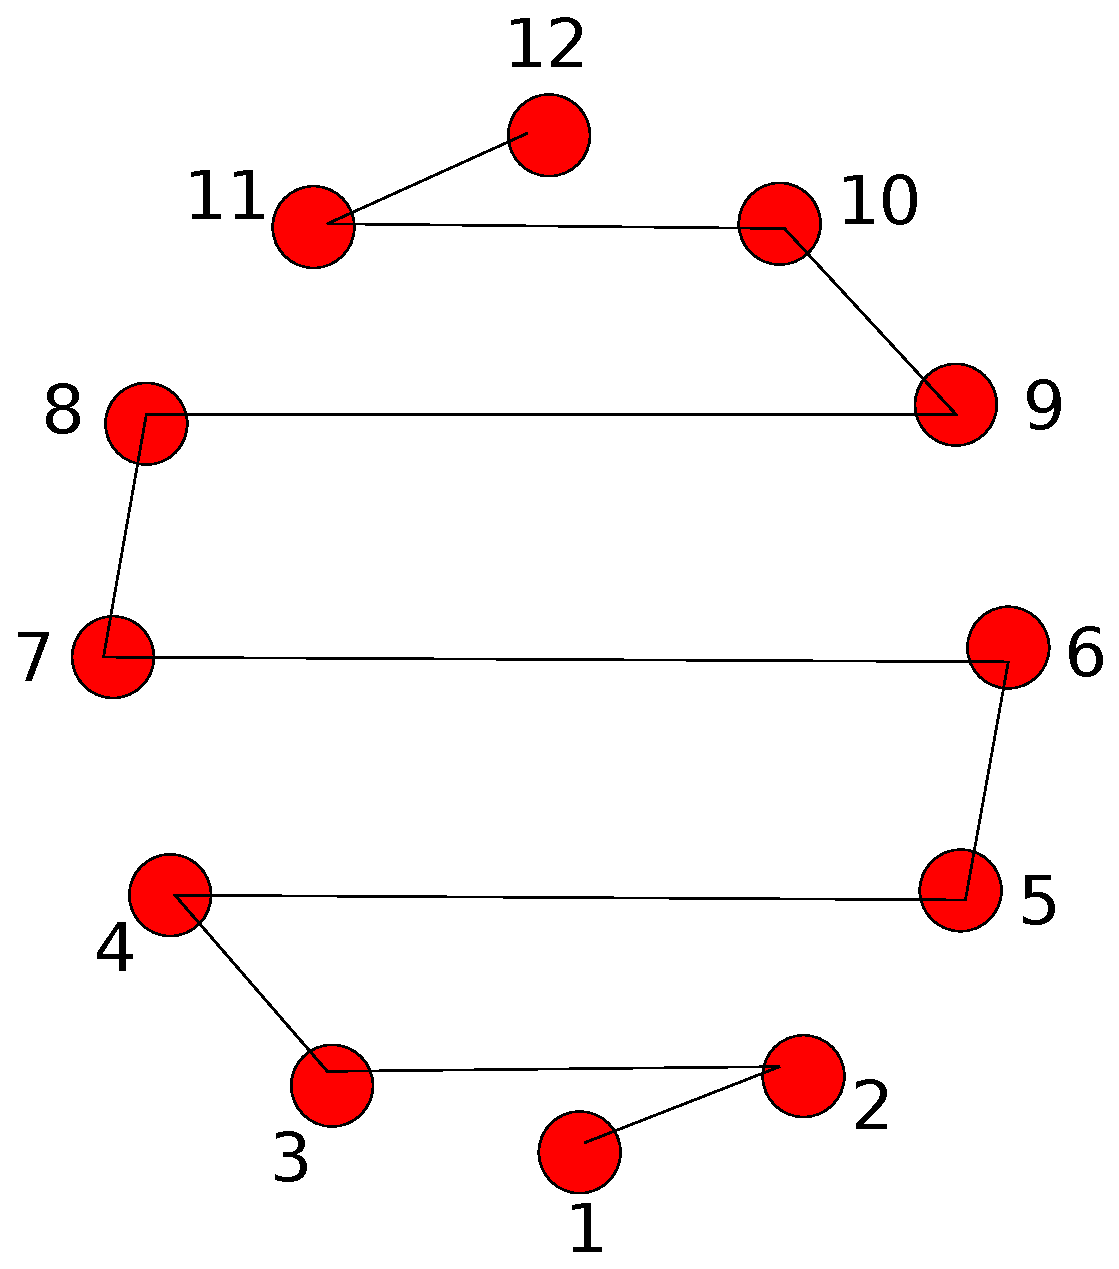
\includegraphics{cyclic.eps}} \end{center} \caption{\emph{Snake-like} ordering of orbitals in a ring-like molecule.} \label{fig:order}
 \end{figure}
%\subsection{Appendix: Orbital ordering}

\subsubsection{Monitoring and convergence of the DMRG calculation}
\label{sec:dmrg_convergence}
%ROA
%In certain cases, a DMRG calculation may become stuck at a local minimum.  To
%ensure that the calculation is converging as $M$ increases along the schedule,
%it is convenient to use the ``discarded weight'' quantity, an estimate of the
%error, in the DMRG calculation.  The discarded weight (DW) converges almost
%linearly as a function of the discarded weight. A strong deviation from this
%(e.g. a plateau behaviour followed by a sudden drop of the energy as a function
%of discarded weight) indicates that the DMRG was stuck in a local minimum. In
%such cases, one can avoid being stuck in the local minimum by increasing the
%amount of noise in the DMRG sweep.

As described in section \ref{sec:appendix1}, a DMRG calculation consists of a
number of sweeps (sweep iterations); each sweep is itself composed of a number
of block iterations equal to $k-4$, where $k$ is the total number of orbitals.
Within a DMRG calculation there are two concepts of convergence. The first is
the convergence to the true FCI energy within the active space, as a function
of the number of renormalised states $M$. The second is the convergence to the
theoretical DMRG energy for a fixed $M$. The first is achieved by going to a
sufficiently large $M$, while the second is achieved by performing a sufficient
number of sweeps for a given $M$ and ensuring that one is not stuck in a local
minimum.

The local minimum problem in DMRG is a nuisance, but in practice can be
avoided.  This is done by checking the convergence of the energy as a function
of $M$.  As a proxy for $M$, it is convenient to use the ``discarded weight''
quantity in the DMRG calculation, which is an estimate of the error of the DMRG
calculation. The discarded weight is more convenient because the energy
converges almost linearly as a function of the discarded weight. A strong
deviation from this (e.g. a plateau behaviour followed by a sudden drop of the
energy as a function of discarded weight) indicates that the DMRG was stuck in
a local minimum. In such cases, one can avoid being stuck in the local minimum
by increasing the amount of noise in the DMRG sweep.

The discarded weight for each sweep is output in a line as follows
\begin{verbatim}
M =   1500   Largest Discarded Weight = 1.358e-06  Sweep Energy =     -75.7850011688
\end{verbatim}

To check a DMRG calculation convergence, carry out the following steps:
\begin{itemize}
\item For every full sweep with a new $M$, note the sweep energy and discarded weight.
\item A reasonable value for the noise is that it should be about 1-10 $\times$ the discarded weight. If the noise
is too large, the DMRG will not converge (and extrapolation will be inaccurate); if it is too small, the calculation
may get stuck.
\item Plot the sweep energy vs. discarded weight. One should observe an almost linear dependence. 
\item If desired, one can extrapolate the sweep energy as a function of the discarded weight using a 
linear relationship. 
\item If a smooth linear behaviour is not observed, then the calculation should be rerun with an increased noise.
\end{itemize}
%As an example of this, we plot the energies and  discarded weights (as obtained from the output) for the Cr$_2$ molecule calculation,
%along with the associated noise settings, with a reasonable noise setting. Here we see the linear dependence of the energy as a function of the discarded weight.
%Also plotted is an example of the same calculation without any noise, where one can observe the plateau-like behaviour, indicating poor convergence.

{\bf Note.  To simplify convergence monitoring, we have implemented a least
squares minimization of the last sweep for each $M$ (we currently use the last
three of these $M$. This enables the user to see how after one is from
convergence.}

\subsubsection{Warm-up Scheme for Large Systems}\label{sec:warmup}
Users who work with large systems may find that the first DMRG sweep, the warm-up sweep, takes much longer time than the subsequent ones using the default settings, sometimes half of the total computation time. This is because the \texttt{BLOCK} code needs to choose proper environment states as the initial guess. 

By default, \texttt{BLOCK} uses the a sophisticated warm-up method based on Wilson renormalisation group. It chooses the lowest-energy states for each possible quantum number in the environment. The scheme ensures good convergence of DMRG, and avoids getting stuck in a local minimum. However, it can take a huge amount of time in finding those environment configurations and building the operators for them. 

The new \texttt{BLOCK} version 1.0.0 introduces an alternative warm-up scheme called local warm-up scheme. In this scheme, the environment states are chosen as the full configuration space of the next X (X=2,3,4) sites and the Hartree-Fock configuration for the rest sites. It can be specified by using the keyword
\begin{verbatim}
warmup local_Xsite
\end{verbatim}
The time to generate the environment states scales O(1) with system size in the local warm-up method, making it very efficient for large systems.

In principle, this scheme works best with localized orbitals. However, for the limited amount of cases we tested, it also works well with active space calculations using canonical orbitals for most needs. A benchmark result is shown in Table~\ref{tab:warmup}.

\begin{table}
\begin{center}
\begin{tabular}{rrr}
\hline
\hline
warm-up scheme& Energy(Hartree)& Wall time (sec)\\
\hline
local\_2site&-770.1730476921&2994\\
local\_3site&-770.1730476961&3061\\
Wilson&-770.1730477013&3545\\
\hline
\hline
\end{tabular}
\end{center}
\caption{
  DMRG converged energies and computation times using 3 different warm-up schemes, tested on C$_{20}$H$_{22}$ molecule with an active space of (20e,20o) using \textbf{canonical orbitals}. All 3 calculations converge after 35 sweeps, with StartM=100, maxM = 1000 and a default schedule. The convergence criteria is $\Delta E<1e-10$ Hartree. The numbers are computed using 4 threads of 2.50GHz Intel Xeon Processor E5-2670.
} \label{tab:warmup}
\end{table}

\subsubsection{Creating FCIDUMP files}\label{sec:appFCIDUMP}
For users who wish to generate their own \texttt{FCIDUMP} file using an external program, the first few lines of \texttt{FCIDUMP} are as follows:
\begin{verbatim}
&FCI NORB=  6
 ORBSYM=1,1,1,1,1,1
&END
   0.692891195085      1  1  1  1
   0.680896658317E-03  2  1  1  1
\end{verbatim}
The first line gives the total number of active orbitals using the keyword \texttt{NORB=}. The second line uses the keyword \texttt{ORBSYM=}, which is followed by the irreducible representation of the active orbitals. The irreps are labelled from 1 to 8 and are given in Table~\ref{tab:irrep}.
Each line following the keyword \texttt{END} has 5 numbers, the first number is the one-electron or two-electron integral and the next 4 integers are the orbital indices. The two body integrals are given in chemists' notation, so a line containing two-body integrals will be\\
\texttt{
\\$( a b|cd)$ a b c d\\}
 
The one-body integrals only need two indices, and the last two indices are just 0 and 0; so a typical line containing one body integral will be\\
\texttt{
\\$\langle a|b\rangle$ a b 0 0\\}

Finally if one is performing an active space calculation, then the core energy can be specified with all four incides equal to 0, e.g.
\begin{verbatim}
core_energy 0 0 0 0
\end{verbatim}

\subsection{Computational considerations}\label{sec:computation}

\begin{itemize}
\item Memory: The scaling of DMRG calculations with the number of states $M$ and orbitals $k$ is roughly $M^2 k^2$.
DMRG calculations are very memory intensive. We recommend systems with at least 4Gb per core, and preferably 8Gb per core. Most
of the DMRG storage is distributed (not replicated) across processors (see Chan (2004) in section \ref{sec:papers} for more details
on the parallelization strategy).

Note that memory fragmentation is an issue in long-running DMRG calculations. This can be simply resolved by stopping the calculation and restarting it.
\item CPU: DMRG CPU times scale as $M^3 k^3$ per sweep. For small $M$ (say, less than 1000), the implementation has a
large $M^2$ overhead which can dominate the computational cost. The total time taken in a calculation can sometimes
be significantly reduced by adjusting the schedule, for example performing more sweeps at smaller $M$.
\item Parallelization: In general, DMRG calculations parallelise well up to a number of cores equal to the number of orbitals. Both
memory and CPU usage is parallelised.
\end{itemize}

For benchmarking, some timing data per sweeps for the Cr$_2$ molecule (see
Section~\ref{sec:cr2}), using 2.67GHz Intel Xeon Processor E5650 is provided in
Table~\ref{tab:timing}, and Table~\ref{tab:thread}.

\begin{table}
\begin{center}
\begin{tabular}{rr}
\hline
\hline
M& Wall time (sec)\\
\hline
500     &567.33\\
1000	&1080.09\\
2000	&2361.30\\
4000	&5056.88\\
6000	&10001.75\\
8000	&17240.69\\
10000	&25964.46\\
\hline
\hline
\end{tabular}
\end{center}
\caption{Wall clock time per sweep for the Cr$_2$ molecule with an active space
of (24e, 30o), using 12 threads of 2.67GHz Intel Xeon Processor E5650. For
these calculations the D$_{2h}$ point group symmetry was used, and a schedule
of size M for all sweeps.
To compare energies, a default schedule run should yield an energy of -2086.42081 Hartree.
} \label{tab:timing}
\end{table}

\begin{table}
\begin{center}
\begin{tabular}{llr}
\hline
\hline
Threads && Wall time (sec)\\
\hline
1 proc &2 core  &18556.01\\
1 proc &4 core  &10191.40\\
1 proc &8 core  &6151.14\\
1 proc &12 core &5056.88\\
2 procs &8 core &3731.93\\
\hline
\hline
\end{tabular}
\end{center}
\caption{Wall clock time per sweep for the Cr$_2$ molecule with an
active space of (24e, 30o), using M=4000 and different amount of
threads of 2.67GHz Intel Xeon Processor E5650. For these calculations
the D$_{2h}$ point group symmetry was used.} \label{tab:thread}
\end{table}


\subsection{Other examples}
In this section we give further example inputs to illustrate
the use of the options above.

\subsubsection{Cr$_2$}\label{sec:cr2}

In J. Chem. Phys. \textbf{136} (2012), 124121, we published a calculation on
the Cr$_2$ molecule using the Ahlrichs SVP basis set and an active space of
(24e, 30o). The molpro input file that was used to generate the integrals is
shown below. 

The \texttt{BLOCK} input file used to calculate the energies in the paper is shown below
\begin{verbatim}
 nelec 24
spin 0
irrep 1

schedule
0 50 1e-5 1e-4
4 250 1e-5 1e-4
8 500 1e-5 1e-5
12 1000 1e-5 1e-5
16 2000 1e-5 1e-5
20 5000 1e-5 1e-5
24 8000 1e-5 1e-5
28 10000 1e-5 1e-5
end
maxiter 31
twodot
sweep_tol 1e-9

orbitals FCIDUMP

reorder reorder.dat

point_group d2h
\end{verbatim}

The reorder.dat file is used to reorder orbitals to place the bonding and anti-bonding orbitals next to each other, i.e. {$\sigma, \sigma^*, \pi_x, \pi_x^*, \pi_y, \pi_y^*, \delta_{xy}, \delta_{xy}^*, \delta_{x^2-y^2}, \delta_{x^2-y^2}^*$}. The reorder.dat file is shown below\\

%\begin{verbatim}
 7,  5,  4,  2,  1,
16, 17, 19, 20, 22,
10,  9,  8, 23, 24,
25, 13, 12, 11, 26,
27, 28, 15, 14, 29,
30,  6,  3, 18, 21            
%\end{verbatim}

\subsubsection{$\pi$-active space of porphine}

We provide a \texttt{MOLPRO} input file for the porphine molecule in Sec.~\ref{sec:PorphineInp}. We localize the $\pi$-orbitals, in a similar fashion to the 
benzene case. We generate a (24e, 24o) active space. The energy is minimized to 
below 0.1 m$E_h$ at M=2000.

\textbf{\texttt{BLOCK} input file}
\begin{verbatim}
nelec 24
point_group c1
spin 0
irrep 1
schedule default
maxm 2000
twodot
sweep_tol 1e-9
orbitals FCIDUMP
gaopt default
\end{verbatim}

\subsection{Appendix: Molpro input files}\label{sec:appMolpro}

 \subsubsection{Benzene molecule}
 \label{sec:appMolprobenz}
\begin{enumerate}

 \item First, a restricted Hartree-Fock calculation is performed. No symmetry
	 is used (\texttt{symmetry,nosym}), because we wish to generate
	 atomic-like $p_z$ orbitals for the DMRG calculation, which requires
	 localizing the orbitals across different irreducible representations. 

In general, the Hartree-Fock orbitals need to be visualized to see which
orbitals should be in the active space. For example, in this calculation, we
find that orbitals 17, 20 and 21 are $\pi$ orbitals, and orbitals 22, 23 and 24
are $\pi*$ orbitals.  At this stage, all the orbitals are delocalized.

%% \begin{figure}
%% \begin{center}
%% \resizebox{80mm}{!}{\includegraphics{orb19.eps}}
%% \end{center}
%% \caption{17$^{th}$ canonical hartree fock molecular orbital of benzene molecule showing the lowest energy $\pi$ orbital.}
%% \label{fig:orb19}
%% \end{figure}

\item We recognize that benzene is a ring-like molecule, and that a good
	orbital choice for the DMRG calculation is the set of localized
	orbitals (section \ref{sec:appendix2}). In Molpro, the orbitals to be
	localized need to be arranged contiguously. We thus exchange the 17th
	orbital with the 19th, using the \texttt{rotate} directive in the
	\texttt{mcscf} program. The \texttt{merge} program is a more robust
	method to localize the orbitals.

%% \begin{figure}
%% \begin{center}
%% \resizebox{80mm}{!}{\includegraphics{orb19_loc.eps}}
%% \end{center}
%% \caption{A localized molecular orbital of benzene molecule obtained by localizing $\pi$ and $\pi^*$ molecular orbitals.}
%% \label{fig:orb19_loc}
%% \end{figure}

\item The six $\pi$ and $\pi^*$ orbitals are localized using the
	\texttt{locali} command, yielding a set of 6 $p_z$ atomic-like
	orbitals. 

\item The \texttt{fci} program is used to dump out one- and two-electron
integrals and information on the irreducible representations of the orbitals.
The resulting file is named \texttt{FCIDUMP}. This contains all the orbital
information required by \texttt{BLOCK}.  \end{enumerate}
{
\begin{verbatim}
angstrom
symmetry, nosym
geomtyp=xyz
geometry={
C  0.000  1.396  0.000
C  1.209  0.698  0.000
C  1.209 -0.698  0.000
C  0.000 -1.396  0.000
C -1.209 -0.698  0.000
C -1.209  0.698  0.000
H  0.000  2.479  0.000
H  2.147  1.240  0.000
H  2.147 -1.240  0.000
H  0.000 -2.479  0.000
H -2.147 -1.240  0.000
H -2.147  1.240  0.000
}
basis=sto-3g
{rhf
wf, 42, 1, 0
}
{mcscf,
occ, 21
frozen, 20
rotate, 19.1, 17.1, 0
}

{locali, pipek, locmethod=3
thresh, 1d-12, 1e-5
core, 18
occ, 24
}

{fci,
core, 18
occ, 24
dump
}
\end{verbatim}
}
\subsubsection{Chromium dimer}
 \label{sec:appMolprocr2}
\begin{verbatim}
basis={
s,CR,0.515280863E+05,0.773721035E+04,0.176037485E+04,0.496877065E+03;
        0.161465206E+03,0.554663523E+02,0.107547330E+03,0.124086719E+02;
        0.504236288E+01,0.854616402E+01,0.139004412E+01,0.560666029E+00;
        0.714837060E-01,0.282506876E-01
c,1.6, 0.144058231E-02, 0.110362023E-01, 0.546766518E-01;
        0.189650381E+00, 0.382954129E+00, 0.290900507E+00
c,7.9,-0.109322811E+00, 0.644725995E+00, 0.462627126E+00
c,10.12,-0.227110133E+00, 0.733015276E+00, 0.442255654E+00
c,13.13, 0.100000000E+01
c,14.14, 0.100000000E+01
p,CR,0.640485361E+03,0.150697112E+03,0.475037553E+02,0.169341202E+02;
        0.624096806E+01,0.308854632E+01,0.117910478E+01,0.433697744E+00
c,1.5, 0.961267152E-02, 0.708898347E-01, 0.270652590E+00, 0.524373434E+00;
        0.341079947E+00
c,6.8, 0.339739869E+00, 0.572720629E+00, 0.245827282E+00
d,CR,0.275594794E+02,0.746870203E+01,0.243459036E+01,0.782447548E+00;
        0.219957743E+00
c,1.4, 0.306124880E-01, 0.155932709E+00, 0.369844213E+00, 0.470711181E+00
c,5.5, 0.339416499E+00
}


geomtyp = xyz
angstrom
geometry={
Cr    0.0 0.0  0.75
Cr    0.0 0.0 -0.75
}

{hf; 
wf,48,1,0; 
occ, 8,3,3,1,5,2,2,0;
}

{fci;
core,4,1,1,0,4,1,1,0;
dump
}
\end{verbatim}

\subsubsection{Porphine, $C_1$ symmetry, fully-localized orbitals}
\label{sec:PorphineInp}

\textbf{molpro input file}

\begin{verbatim}
angstrom
geomtyp = xyz
geometry = {
N 1.9764 0.0000 0.0000
N 0.0000 1.9884 0.0000
N -1.9764 0.0000 0.0000
N 0.0000 -1.9884 0.0000
C 2.8182 -1.0903 0.0000
C 2.8182 1.0903 0.0000
C 1.0918 2.8249 0.0000
C -1.0918 2.8249 0.0000
C -2.8182 1.0903 0.0000
C -2.8182 -1.0903 0.0000
C -1.0918 -2.8249 0.0000
C 1.0918 -2.8249 0.0000
C 4.1961 -0.6773 0.0000
C 4.1961 0.6773 0.0000
C 0.6825 4.1912 0.0000
C -0.6825 4.1912 0.0000
C -4.1961 0.6773 0.0000
C -4.1961 -0.6773 0.0000
C -0.6825 -4.1912 0.0000
C 0.6825 -4.1912 0.0000
H 5.0441 -1.3538 0.0000
H 5.0441 1.3538 0.0000
H 1.3558 5.0416 0.0000
H -1.3558 5.0416 0.0000
H -5.0441 1.3538 0.0000
H -5.0441 -1.3538 0.0000
H -1.3558 -5.0416 0.0000
H 1.3558 -5.0416 0.0000
C 2.4150 2.4083 0.0000
C -2.4150 2.4083 0.0000
C -2.4150 -2.4083 0.0000
C 2.4150 -2.4083 0.0000
H 3.1855 3.1752 0.0000
H -3.1855 3.1752 0.0000
H -3.1855 -3.1752 0.0000
H 3.1855 -3.1752 0.0000
}
basis=vdz
gprint, orbital= 500
{rhf
core 0,0,0,0,0,0,0,0
}

symmetry, nosym
{rhf
maxit, 1
start, 2100.2
save, 2101.2
print, orbital=500
}

{merge
orbital, 2101.2
add 1.1,396.1,1.1
rotate 70.1, 73.1, 90
rotate 68.1, 72.1, 90
rotate 62.1, 71.1, 90
rotate 61.1, 70.1, 90
rotate 58.1, 69.1, 90
rotate 92.1, 85.1, 90
rotate 94.1, 86.1, 90
rotate 95.1, 87.1, 90
rotate 96.1, 88.1, 90
rotate 101.1, 89.1, 90
rotate 102.1, 90.1, 90
rotate 103.1, 91.1, 90
rotate 104.1, 92.1, 90
save 2102.2
}

{rhf;
start 2102.2
maxit, 1
save 2103.2
}

{locali, pipek, locmethod=3
orbital,  2103.2
thresh, 1d-12, 1e-5
core, 68
occ,  92
save, 2104.2
}

{fci
orbital, 2105.2
core, 68
occ,  92
dump
}
\end{verbatim}

\end{document}
